%%%%%%%%%%%%%%%%%%%%%%%%%%%%% Define Article %%%%%%%%%%%%%%%%%%%%%%%%%%%%%%%%%%
\documentclass{article}
%%%%%%%%%%%%%%%%%%%%%%%%%%%%%%%%%%%%%%%%%%%%%%%%%%%%%%%%%%%%%%%%%%%%%%%%%%%%%%%

%%%%%%%%%%%%%%%%%%%%%%%%%%%%% Using Packages %%%%%%%%%%%%%%%%%%%%%%%%%%%%%%%%%%
\usepackage{geometry}
\usepackage{graphicx}
\usepackage{amssymb}
\usepackage{amsmath}
\usepackage{tikz}
\usepackage{tcolorbox}
\usepackage{listings}
%%%%%%%%%%%%%%%%%%%%%%%%%%%%%%%%%%%%%%%%%%%%%%%%%%%%%%%%%%%%%%%%%%%%%%%%%%%%%%%

% Other Settings

%%%%%%%%%%%%%%%%%%%%%%%%%% Page Setting %%%%%%%%%%%%%%%%%%%%%%%%%%%%%%%%%%%%%%%
% \geometry{a4paper}

%%%%%%%%%%%%%%%%%%%%%%%%%% Define some useful colors %%%%%%%%%%%%%%%%%%%%%%%%%%
\definecolor{ocre}{RGB}{243,102,25}
\definecolor{mygray}{RGB}{243,243,244}
\definecolor{deepGreen}{RGB}{26,111,0}
\definecolor{shallowGreen}{RGB}{235,255,255}
\definecolor{deepBlue}{RGB}{61,124,222}
\definecolor{shallowBlue}{RGB}{235,249,255}

\definecolor{codegreen}{rgb}{0,0.6,0}
\definecolor{codegray}{rgb}{0.5,0.5,0.5}
\definecolor{codepurple}{rgb}{0.58,0,0.82}
\definecolor{backcolour}{rgb}{0.95,0.95,0.92}

\lstdefinestyle{mystyle}{
    backgroundcolor=\color{backcolour},   
    commentstyle=\color{codegreen},
    keywordstyle=\color{codepurple},
    numberstyle=\tiny\color{codegray},
    stringstyle=\color{blue},
    basicstyle=\ttfamily\footnotesize,
    breakatwhitespace=false,         
    breaklines=false,                 
    captionpos=b,                    
    keepspaces=false,                 
    numbers=left,                    
    numbersep=0pt,                  
    showspaces=false,                
    showstringspaces=false,
    showtabs=false,                  
    tabsize=1
}

\lstset{style=mystyle, language=Python}
%%%%%%%%%%%%%%%%%%%%%%%%%%%%%%%%%%%%%%%%%%%%%%%%%%%%%%%%%%%%%%%%%%%%%%%%%%%%%%%

%%%%%%%%%%%%%%%%%%%%%%%%%% Define some useful commands %%%%%%%%%%%%%%%%%%%%%%%%
\newcommand{\fig}[3][1.0]{
    \begin{figure}[!ht]
        \centering
        \includegraphics[width=#1\linewidth]{#2}
        \caption{#3}
        \label{fig:#2}
    \end{figure}
}

\newcommand{\reffig}[1]{Fig. \ref{fig:#1}}

%%%%%%%%%%%%%%%%%%%%%%%%%% Define an orangebox command %%%%%%%%%%%%%%%%%%%%%%%%
% \newcommand\orangebox[1]{\fcolorbox{ocre}{mygray}{\hspace{1em}#1\hspace{1em}}}
%%%%%%%%%%%%%%%%%%%%%%%%%%%%%%%%%%%%%%%%%%%%%%%%%%%%%%%%%%%%%%%%%%%%%%%%%%%%%%%

%%%%%%%%%%%%%%%%%%%%%%%%%%%% English Environments %%%%%%%%%%%%%%%%%%%%%%%%%%%%%
% \newtheoremstyle{mytheoremstyle}{3pt}{3pt}{\normalfont}{0cm}{\rmfamily\bfseries}{}{1em}{{\color{black}\thmname{#1}~\thmnumber{#2}}\thmnote{\,--\,#3}}
% \newtheoremstyle{myproblemstyle}{3pt}{3pt}{\normalfont}{0cm}{\rmfamily\bfseries}{}{1em}{{\color{black}\thmname{#1}~\thmnumber{#2}}\thmnote{\,--\,#3}}
% \theoremstyle{mytheoremstyle}
% \newmdtheoremenv[linewidth=1pt,backgroundcolor=shallowGreen,linecolor=deepGreen,leftmargin=0pt,innerleftmargin=20pt,innerrightmargin=20pt,]{theorem}{Theorem}[section]
% \theoremstyle{mytheoremstyle}
% \newmdtheoremenv[linewidth=1pt,backgroundcolor=shallowBlue,linecolor=deepBlue,leftmargin=0pt,innerleftmargin=20pt,innerrightmargin=20pt,]{definition}{Definition}[section]
% \theoremstyle{myproblemstyle}
% \newmdtheoremenv[linecolor=black,leftmargin=0pt,innerleftmargin=10pt,innerrightmargin=10pt,]{problem}{Problem}[section]
%%%%%%%%%%%%%%%%%%%%%%%%%%%%%%%%%%%%%%%%%%%%%%%%%%%%%%%%%%%%%%%%%%%%%%%%%%%%%%%

%%%%%%%%%%%%%%%%%%%%%%%%%%%%%%% Title & Author %%%%%%%%%%%%%%%%%%%%%%%%%%%%%%%%
\title{Detección PPM}
\author{Armando Palacio Romeu}
%%%%%%%%%%%%%%%%%%%%%%%%%%%%%%%%%%%%%%%%%%%%%%%%%%%%%%%%%%%%%%%%%%%%%%%%%%%%%%%

\begin{document}
\maketitle

\section{Introducción}
    En este breve articulo se resumirá toda la deducción teórica de los distintos métodos de detección para 
    señales PPM. Se abordarán los métodos de decisión blanda y dura, así como la deducción de la probabilidad de error de símbolo
    y probabilidad de error de bit para cada uno de los métodos. 

\section{Soft Decision, Maximun a posteriori (MAP)}
    La decisión blanda se basa en el criterio de máximo a posteriori (MAP), en el cual se minimiza la 
    probabilidad de error de símbolo (SER). Suponiendo el caso general M-ary PPM los símbolos base se 
    pueden representar como $\vec{s}_i = \mu_1 \vec{e}_i$ con $i = 1,2,\dots,M$ y 
    $\vec{e}_i$ son los vectores unitarios del espacio vectorial $\mathbb{R}^M$. Es decir,
    los vectores $\vec{s}_i$ son ortogonales entre sí. Todos los símbolos $\vec{s}_i$ son igualmente 
    probables, por lo que $P(\vec{s}_i) = \frac{1}{M}$ para todo $i$.

    \underline{Vector recibido:} 
    \begin{equation}
        \vec{y} = \vec{s} + \vec{w}, \quad \vec{y} = [y_1,y_2,\dots,y_M]^T, \quad \vec{s} = [s_1,s_2,\dots,s_M]^T, \quad \vec{w} = [w_1,w_2,\dots,w_M]^T
    \end{equation}
    donde $\vec{w}\in \mathbb{R}^M$ es el vector de ruido que es añadido tanto por el amplificador 
    óptico (ruido ASE) como por el fotodetector (ruido térmico y \textit{Shot}). Este ruido se
    puede modelar como un proceso aleatorio gaussiano de media cero y matriz de covarianza $\mathbb{K}$ 
    ($\vec{w}\sim \mathcal{N}(\vec{0},\mathbb{K} )$). 

    \underline{Tets de hipotesis:}
    \begin{equation}
        f(\vec{y}|\vec{s}_i) 
        \begin{array}{c}
            H_i \\
            \gtrless \\
            H_j
        \end{array}
        f(\vec{y}|\vec{s}_j) \quad \forall i,j \in \{1,2,\dots,M\}, \quad i\neq j, \quad
        \begin{cases}
            H_i: \vec{s}_i \text{  was sent} \\
            H_j: \vec{s}_j \text{  was sent}
        \end{cases}
    \end{equation}

    \underline{Log-liklihood:}
    \begin{equation}
        \Lambda_{ij}(\vec{y}) = \ln \left( \frac{f(\vec{y}|\vec{s}_i)}{f(\vec{y}|\vec{s}_j)} \right) 
        \begin{array}{c}
            H_i \\
            \gtrless \\
            H_j
        \end{array}
        0 \label{log-liklihood}
    \end{equation}

    La varianza del ruido es diferente para los slots \textbf{0} y \textbf{1} por lo que
    la matriz de covarianza $\mathbb{K}$ es diferente para cada símbolo $\vec{s}_i$ y se puede expresar como:
    \begin{align}
        &\mathbb{K}_{\vec{s}_i} = 
        \begin{bmatrix}
            \sigma_{0}^2 & \dots & 0 & \dots & 0 \\
            \vdots & \ddots & \vdots & \dots & \vdots \\
            0 & \dots & \sigma_1^2 & \dots & 0 \\
            \vdots & \dots & \vdots & \ddots & \vdots \\
            0 & \dots & 0 & \dots & \sigma_{0}^2
        \end{bmatrix} \nonumber\\
        &\mathbb{K}_{\vec{s}_i}[m,m] = \sigma_0^2 \quad \forall m\in\{1,2,\dots,M\}, \quad m\neq i \nonumber\\ 
        &\mathbb{K}_{\vec{s}_i}[i,i] = \sigma_1^2
    \end{align}
    El determinante de esta matríz es $\det(\mathbb{K}_{\vec{s}_i}) = \sigma_0^{2(M-1)}\sigma_1^2$
    el cual es igual para todos los símbolos $\vec{s}_i$. Entonces se puede expresar la densidad de probabilidad del vector recibido $\vec{y}$ como:

    \begin{equation}
        f(\vec{y}|\vec{s}_i) = \frac{1}{(2\pi)^{M/2}\sqrt{\det(\mathbb{K}_{\vec{s}_i})}}\exp\left( -\frac{1}{2}(\vec{y}-\vec{s}_i)^T\mathbb{K}_{\vec{s}_i}^{-1}(\vec{y}-\vec{s}_i) \right)
    \end{equation}
    donde $\mathbb{K}^{-1}$ es la inversa de la matriz $\mathbb{K}$ y se puede expresar como:
    \begin{equation}
        \mathbb{K}_{\vec{s}_i}^{-1} = 
        \begin{bmatrix}
            \frac{1}{\sigma_0^2} & \dots & 0 & \dots & 0 \\
            \vdots & \ddots & \vdots & \dots & \vdots \\
            0 & \dots & \frac{1}{\sigma_1^2} & \dots & 0 \\
            \vdots & \dots & \vdots & \ddots & \vdots \\
            0 & \dots & 0 & \dots & \frac{1}{\sigma_{0}^2}
        \end{bmatrix}
    \end{equation}

    Regresando a la Ec. \ref{log-liklihood} queda:
    \begin{align}
        \Lambda_{ij}(\vec{y}) &= -\frac{1}{2}(\vec{y}-\vec{s}_i)^T\mathbb{K}_{\vec{s}_i}^{-1}(\vec{y}-\vec{s}_i) + \frac{1}{2}(\vec{y}-\vec{s}_j)^T\mathbb{K}_{\vec{s}_j}^{-1}(\vec{y}-\vec{s}_j) \nonumber\\
        &= \frac{1}{2} \left( -\frac{(y_i-\mu_1)^2}{\sigma_1^2} - \frac{y_j^2}{\sigma_0^2} + \frac{y_i^2}{\sigma_0^2} + \frac{(y_j-\mu_1)^2}{\sigma_1^2} \right) \nonumber\\
        &= \frac{1}{2} \left( \frac{1}{\sigma_1^2}\left[(y_j-\mu_1)^2-(y_i-\mu_1)^2\right] + \frac{1}{\sigma_0^2}\left[y_i^2-y_j^2\right]  \right) \nonumber\\
        &= \frac{1}{2} \left( \left[ \frac{1}{\sigma_0^2} - \frac{1}{\sigma_1^2} \right](y_i-y_j)^2 + \frac{2\mu_1}{\sigma_1^2}(y_i-y_j)  \right) \nonumber\\
        &= \frac{1}{2} \left( \left[ \frac{1}{\sigma_0^2} - \frac{1}{\sigma_1^2} \right](y_i+y_j) + \frac{2\mu_1}{\sigma_1^2}  \right)(y_i-y_j)
        \begin{array}{c}
            H_i \\
            \gtrless \\
            H_j
        \end{array} 0 
    \end{align}

    Esta expresión nos revela dos condiciones:
    \begin{enumerate}
        \item $\left( \left[ \frac{1}{\sigma_0^2} - \frac{1}{\sigma_1^2} \right](y_i+y_j) + \frac{2\mu_1}{\sigma_1^2}  \right) \begin{array}{c}
            H_i \\
            \gtrless \\
            H_j
        \end{array} 0 \quad \Longrightarrow \quad 
        y_i+y_j \begin{array}{c}
            H_i \\
            \gtrless \\
            H_j
        \end{array} -\frac{2\mu_1\sigma_0^2}{\sigma_1^2-\sigma_0^2} $
        
        \item $(y_i-y_j) \begin{array}{c}
            H_i \\
            \gtrless \\
            H_j
        \end{array} 0 \quad \Longrightarrow \quad
        y_i \begin{array}{c}
            H_i \\
            \gtrless \\
            H_j
        \end{array} y_j$
    \end{enumerate}

    La primera condición no tiene sentido físico. En cambio la segunda condición
    nos dice que si $y_i$ es mayor que $y_j$ entonces el símbolo transmitido fue $\vec{s}_i$,
    de lo contrario el símbolo transmitido fue $\vec{s}_j$. Teniendo en cuenta que esta condición 
    debe verificarse para $\forall i,j \in \{1,2,\dots,M\}, \quad i\neq j$ se puede concluir que
    el estimador de máxima verosimilitud para el símbolo transmitido es: 
    \begin{equation}
        \hat{\vec{s}} = \vec{s}_{\arg \max \{y_k\}}
    \end{equation}


    \subsection{Probabilidad de error de símbolo}
        Existen dos formas de expresar la probabilidad de error de símbolo a partir de la condición
        obtenida anteriormente.

        \subsubsection{Cálculo a partir de todos los eventos que provocan un error}
            Para que se entienda mejor explicaré este apartado asumiento que $M=4$ y que se transmitió $\vec{s}_1$,
            más adelante se generalizará el resultado.
            Los posibles eventos que provocan un error de símbolo son:
            \begin{itemize}
                \item[A)] $y_2 > y_1, \quad y_3,y_4<y_1, \quad$ 
                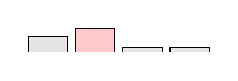
\begin{tikzpicture}[baseline=(current bounding box.center)]
                    \draw[fill=gray!20] (0,0) -- (0,0.2) -- (0.5,0.2) -- (0.5,0);
                    \draw[fill=red!20] (0.6,0) -- (0.6,0.3) -- (1.1,0.3) -- (1.1,0);
                    \draw[fill=gray!20] (1.2,0) -- (1.2,0.05) -- (1.7,0.05) -- (1.7,0);
                    \draw[fill=gray!20] (1.8,0) -- (1.8,0.05) -- (2.3,0.05) -- (2.3,0);
                \end{tikzpicture}
                \item[B)] $y_3 > y_1, \quad y_2,y_4<y_1, \quad$
                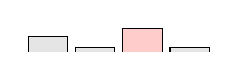
\begin{tikzpicture}[baseline=(current bounding box.center)]
                    \draw[fill=gray!20] (0,0) -- (0,0.2) -- (0.5,0.2) -- (0.5,0);
                    \draw[fill=gray!20] (0.6,0) -- (0.6,0.05) -- (1.1,0.05) -- (1.1,0);
                    \draw[fill=red!20] (1.2,0) -- (1.2,0.3) -- (1.7,0.3) -- (1.7,0);
                    \draw[fill=gray!20] (1.8,0) -- (1.8,0.05) -- (2.3,0.05) -- (2.3,0);
                \end{tikzpicture}
                \item[C)] $y_4 > y_1, \quad y_2,y_3<y_1, \quad$
                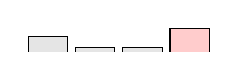
\begin{tikzpicture}[baseline=(current bounding box.center)]
                    \draw[fill=gray!20] (0,0) -- (0,0.2) -- (0.5,0.2) -- (0.5,0);
                    \draw[fill=gray!20] (0.6,0) -- (0.6,0.05) -- (1.1,0.05) -- (1.1,0);
                    \draw[fill=gray!20] (1.2,0) -- (1.2,0.05) -- (1.7,0.05) -- (1.7,0);
                    \draw[fill=red!20] (1.8,0) -- (1.8,0.3) -- (2.3,0.3) -- (2.3,0);
                \end{tikzpicture}
                \item[D)] $y_2,y_3 > y_1, \quad y_4<y_1, \quad$
                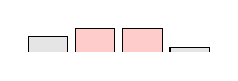
\begin{tikzpicture}[baseline=(current bounding box.center)]
                    \draw[fill=gray!20] (0,0) -- (0,0.2) -- (0.5,0.2) -- (0.5,0);
                    \draw[fill=red!20] (0.6,0) -- (0.6,0.3) -- (1.1,0.3) -- (1.1,0);
                    \draw[fill=red!20] (1.2,0) -- (1.2,0.3) -- (1.7,0.3) -- (1.7,0);
                    \draw[fill=gray!20] (1.8,0) -- (1.8,0.05) -- (2.3,0.05) -- (2.3,0);
                \end{tikzpicture}
                \item[E)] $y_2,y_4 > y_1, \quad y_3<y_1, \quad$
                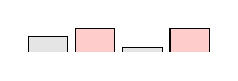
\begin{tikzpicture}[baseline=(current bounding box.center)]
                    \draw[fill=gray!20] (0,0) -- (0,0.2) -- (0.5,0.2) -- (0.5,0);
                    \draw[fill=red!20] (0.6,0) -- (0.6,0.3) -- (1.1,0.3) -- (1.1,0);
                    \draw[fill=gray!20] (1.2,0) -- (1.2,0.05) -- (1.7,0.05) -- (1.7,0);
                    \draw[fill=red!20] (1.8,0) -- (1.8,0.3) -- (2.3,0.3) -- (2.3,0);
                \end{tikzpicture}
                \item[F)] $y_3,y_4 > y_1, \quad y_2<y_1, \quad$
                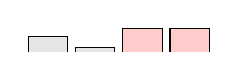
\begin{tikzpicture}[baseline=(current bounding box.center)]
                    \draw[fill=gray!20] (0,0) -- (0,0.2) -- (0.5,0.2) -- (0.5,0);
                    \draw[fill=gray!20] (0.6,0) -- (0.6,0.05) -- (1.1,0.05) -- (1.1,0);
                    \draw[fill=red!20] (1.2,0) -- (1.2,0.3) -- (1.7,0.3) -- (1.7,0);
                    \draw[fill=red!20] (1.8,0) -- (1.8,0.3) -- (2.3,0.3) -- (2.3,0);
                \end{tikzpicture}
                \item[G)] $y_2,y_3,y_4 > y_1, \quad\quad\quad\quad\:$
                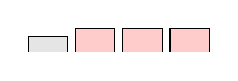
\begin{tikzpicture}[baseline=(current bounding box.center)]
                    \draw[fill=gray!20] (0,0) -- (0,0.2) -- (0.5,0.2) -- (0.5,0);
                    \draw[fill=red!20] (0.6,0) -- (0.6,0.3) -- (1.1,0.3) -- (1.1,0);
                    \draw[fill=red!20] (1.2,0) -- (1.2,0.3) -- (1.7,0.3) -- (1.7,0);
                    \draw[fill=red!20] (1.8,0) -- (1.8,0.3) -- (2.3,0.3) -- (2.3,0);
                \end{tikzpicture}
            \end{itemize}
            La distribución de amplitudes del slot $y_1$ se puede expresar como:

            \begin{equation}
                f_{y_1}(x) = \frac{1}{\sqrt{2\pi\sigma_1^2}}e^{-\frac{1}{2}\left( \frac{x-\mu_1}{\sigma_1} \right)^2}
            \end{equation}
            Para los slots restantes la distribución de amplitudes es la misma y se puede expresar como:
            
            \begin{equation}
                f_{y_k}(x) = \frac{1}{\sqrt{2\pi\sigma_0^2}}e^{-\frac{1}{2}\left( \frac{x}{\sigma_0} \right)^2}
            \end{equation}
            Con estas distribuciones de amplitudes se puede determinar la probabilidad de cada evento $y_k>y_1$ y $y_k<y_1$ como:
            
            \begin{equation}
                P(y_k>y_1) = \int_{y_1}^{\infty} f_{y_k}(x)\:dx= \frac{1}{2}\text{erfc}\left( \frac{y_1}{\sqrt{2}\sigma_0} \right)
            \end{equation}
            \begin{equation}
                P(y_k<y_1) = \int_{-\infty}^{y1} f_{y_k}(x)\:dx= 1-\frac{1}{2}\text{erfc}\left( \frac{y_1}{\sqrt{2}\sigma_0} \right)
            \end{equation}
            Estas probabilidades solo me hablan de que tan probable es que la amplitud del slot $y_k$ sea 
            mayor o menor que la amplitud del slot $y_1$. Si definimos la función $Q(x)$ como:
            
            \begin{equation}
                Q(x) = \frac{1}{2}\text{erfc}\left( \frac{x}{\sqrt{2}} \right)
            \end{equation}
            luego podemos expresar la probabilidad de que la amplitud del slot $y_k$ sea mayor o menor que la amplitud del slot $y_1$ como:
            
            \begin{equation}
                P(y_k>y_1) = Q\left( \frac{y_1}{\sigma_0} \right)
            \end{equation}
            \begin{equation}
                P(y_k<y_1) = 1-Q\left( \frac{y_1}{\sigma_0} \right) = Q\left( -\frac{y_1}{\sigma_0} \right)
            \end{equation}
            Ahora podemos calcular la probabilidad de cada evento $A,B,C,D,E,F,G$ como:
            
            \begin{align}
                P(A,y_1)=P(B,y_1)=P(C,y_1) & = Q\left( \frac{y_1}{\sigma_0} \right) \left[ 1-Q\left( \frac{y_1}{\sigma_0} \right) \right]^2 \\
                P(D,y_1)=P(E,y_1)=P(F,y_1) & = Q\left( \frac{y_1}{\sigma_0} \right)^2 \left[ 1-Q\left( \frac{y_1}{\sigma_0} \right) \right] \\
                P(G,y_1) & = Q\left( \frac{y_1}{\sigma_0} \right)^3
            \end{align}
            Podemos expresar entonces la probabilidad de error de símbolo como la suma de todas las probabilidades anteriores
            integradas por cada valor posible de $y_1$:
            \begin{equation}
                \text{SER} = \int_{-\infty}^{\infty} \left[ 3 P(A,y_1) + 3 P(D,y_1) + P(G,y_1) \right] f_{y_1}(y_1)\:dy_1
            \end{equation}

            Esta expresión se puede generalizar para cualquier $M$ teniendo en cuenta que la cantidad de eventos con la misma probabilidad 
            viene dada por la combinatoria de $M-1$ slots en $k$ slots que son mayores a $y_i$ transmitido. En el caso anterior de $M=4$, 
            la cantidad de eventos con la misma probabilidad cuando un único slot es mayor a $y_1$ es $C_1^3=3$, cuando dos slots son mayores a $y_1$
            es $C_2^3=3$ y cuando los tres slots son mayores a $y_1$ es $C_3^3=1$. Además las probabilidades $P(y_k>y_1)$ y $P(y_k<y_1)$
            quedan pesadas en el exponente por el número de slots que cumplen la condición. Por lo tanto la probabilidad de error de símbolo generalizada 
            para cualquier $M$ se puede expresar como:
            \begin{tcolorbox}[colback=yellow!20!white,colframe=black]
                \begin{align}
                    \text{SER} &= \frac{1}{\sqrt{2\pi\sigma_1^2}} \sum_{k=0}^{M-1} \binom{M-1}{k}\int_{-\infty}^{\infty} Q\left( \frac{x}{\sigma_0} \right)^k \left(1-Q\left( \frac{x}{\sigma_0} \right)\right)^{M-k-1} \exp\left(-\frac{(x-\mu_1)^2}{2\sigma_1}\right)\:dx 
                \end{align}
            \end{tcolorbox}
            
        \subsubsection{Cálculo a partir de los eventos que aseguran el éxito}
            Una forma más sencilla y que brinda una expresión analítica más simple es teniendo en cuenta 
            los sucesos que aseguran el éxito en la detección del símbolo. Considerando nuevamente el caso
            de $M=4$ slots y sabiendo que el símbolo $\vec{s}_1$ fue transmitido, los eventos que aseguran el éxito son:
            
            \begin{itemize}
                \item[A')] $y_2,y_3,y_4 < y_1$ todas las amplitudes de los slots restantes son menores a $y_1$. 
            \end{itemize}
            Entonces la probabilidad de éxito no es más que la probabilidad del evento $A'$ integrada para cada valor de $y_1$, que se puede expresar como:
            
            \begin{equation}
                P(A') = \int_{-\infty}^{\infty}P(y_k<y_1)^{M-1} f_{y_1}(y_1)\:dy_1 = \int_{-\infty}^{\infty}\left[1-Q\left( \frac{y_1}{\sigma_0} \right)\right]^{M-1}f_{y_1}(y_1)\:dy_1
            \end{equation}
            Entonces la probabilidad de error de símbolo es:
            
            \begin{tcolorbox}[colback=yellow!20!white,colframe=black]
                \begin{equation}
                    \text{SER} = 1-P(A') = 1-\frac{1}{\sqrt{2\pi}}\int_{-\infty}^{\infty} \left[1-Q\left( \frac{\mu_1 + \sigma_1 x}{\sigma_0} \right)\right]^{M-1} e^{-x^2/2}\:dx
                \end{equation}
            \end{tcolorbox}
            
            
\section{Hard Decision, Threshold detection}
    Esta forma de detección consiste en comparar la amplitud de cada slot con un umbral $r$
    y asignar un \textbf{1} si el valor supera el umbral, de lo contrario se asignará
    \textbf{0} al slot. En este caso es conveniente definir dos probabilidades auxiliares que serán de utilidad
    para determinar la probabilidad de error de símbolo. La probabilidad de detección de slot,
    que es la probabilidad de que el slot sea detectado como \textbf{1} cuando se transmitió un \textbf{1}:
    \begin{equation}
        P_{D} = P(y>r|x=1) = \frac{1}{\sqrt{2\pi\sigma_1^2}}\int_{r}^{\infty} e^{-\frac{(y-\mu_1)^2}{2\sigma_1^2}}\:dy=Q\left(\frac{r-\mu_1}{\sigma_1}\right)
    \end{equation}
    
    Por otra parte la probabilidad de falsa alarma de slot, que es la probabilidad de que el slot sea detectado como \textbf{1} cuando se transmitió un \textbf{0}:
    \begin{equation}
        P_{FA} = P(y>r|x=0) = \frac{1}{\sqrt{2\pi\sigma_0^2}}\int_{r}^{\infty} e^{-\frac{(y-\mu_0)^2}{2\sigma_0^2}}\:dy=Q\left(\frac{r-\mu_0}{\sigma_0}\right)
    \end{equation}
    
    A partir de estas dos probabilidades se puede determinar la probabilidad de error de símbolo como 
    uno menos la probabilidad de éxito. La probabilidad de éxito es la probabilidad de que todos los slots sean detectados correctamente,
    es decir, que todos los slots sean detectados como \textbf{1} cuando se transmitió un \textbf{1} y como \textbf{0} cuando se transmitió un \textbf{0}.
    Entonces la probabilidad de éxito es:
    \begin{equation}
        P_\text{éxito} = P_{D}(1-P_{FA})^{M-1}
    \end{equation}
    
    Por lo tanto la probabilidad de error de símbolo es:
    \begin{tcolorbox}[colback=yellow!20!white,colframe=black]
        \begin{equation}
            \text{SER}(r) = 1-P_\text{éxito} = 1-P_{D}(1-P_{FA})^{M-1}=1-Q\left(\frac{r-\mu_1}{\sigma_1}\right)\left[1-Q\left(\frac{r-\mu_0}{\sigma_0}\right)\right]^{M-1}
        \end{equation}
    \end{tcolorbox}

    \subsection{Optimum Threshold}
        El umbral óptimo se puede obtener minimizando la probabilidad de error de símbolo. Para ello se deriva la probabilidad de error de símbolo con respecto a $r$ y se iguala a cero.
        
        \begin{align}
            \frac{d \text{SER}(r)}{dr} = \frac{d}{dr}\left[1-Q\left(\frac{r-\mu_1}{\sigma_1}\right)\left[1-Q\left(\frac{r-\mu_0}{\sigma_0}\right)\right]^{M-1}\right] = 0 \nonumber\\
            \frac{dQ_1}{dr}-(M-1)\frac{Q_1}{1-Q_0}\frac{dQ_0}{dr} = 0
            \label{dP_dr}
        \end{align}
        donde $Q_1 = Q\left(\frac{r-\mu_1}{\sigma_1}\right)$ y $Q_0 = Q\left(\frac{r-\mu_0}{\sigma_0}\right)$. Se puede demostrar que el término $Q_1/(1-Q_0)\approx 1$ para valores del umbral cercanos al óptimo. En la fig.~\ref{fig:SER} se muestra, en la primera parcela esta relación y en la segunda parcela la probabilidad de error de símbolo, donde se puede apreciar la aproximación realizada previamente.
        
        \fig{SER}{Apreciación gráfica de la aproximación $Q_1/(1-Q_0)\approx 1$ en la región cercana al umbral óptimo. Para esta simulación se utilizó $\mu_0=0$, $\mu_1=1$, $\sigma_0=0.08$, $\sigma_1=0.11$ y $M=8$.}

        De esta forma la ecuación (\ref{dP_dr}) se simplifica a:
        \begin{align}
            \frac{dQ_1}{dr}-(M-1)\frac{dQ_0}{dr} = 0 \label{dQ_dr}
        \end{align}
        Las derivadas de las funciones Q se pueden obtener de la siguiente forma:
        
        \begin{align}
            \frac{dQ_i}{dr} = \frac{d}{dr}\left[\frac{1}{\sqrt{2\pi\sigma_i^2}}\int_{r}^{\infty} e^{-\frac{(x-\mu_i)^2}{2\sigma_i^2}}\:dx\right] = -\frac{1}{\sigma_i\sqrt{2\pi}}e^{-\frac{(r-\mu_i)^2}{2\sigma_i^2}}
        \end{align}
        Tomando logaritmo natural en ambos miembros de la ecuación (\ref{dQ_dr}) y sustituyendo
        las derivadas de las funciones Q se obtiene:
        
        \begin{align}
            2\ln\left[\frac{\sigma_1}{\sigma_0}(M-1)\right] = -\frac{(r-\mu_1)^2}{\sigma_1^2}+\frac{(r-\mu_0)^2}{\sigma_0^2}
        \end{align}
        Resolviendo la ecuación cuarática resultante para $r$ se obtiene una muy buena aproximación al umbral óptimo. La solución analítica se puede expresar como:
        \begin{tcolorbox}[colback=yellow!20!white,colframe=black]
            \[
            r_{opt} \approx
            \begin{cases}
                \frac{1}{\sigma_1^2-\sigma_0^2}\left(\mu_0\sigma_1^2-\mu_1\sigma_0^2+\sigma_0\sigma_1\sqrt{(\mu_1-\mu_0)^2+2(\sigma_1^2-\sigma_0^2)\ln\left[\frac{\sigma_1}{\sigma_0}(M-1)\right]}\right),
                & \text{si } \sigma_0\neq\sigma_1\\
                \frac{\mu_1+\mu_0}{2} + \frac{\sigma^2}{\mu_1-\mu_0}\ln(M-1), & \text{si } \sigma_0=\sigma_1
            \end{cases}
            \]
        \end{tcolorbox}
        Las \reffig{threshold} y \reffig{threshold_s1_igual_s0} muestran
        las soluciones analíticas obtenidas a partir de Wolfram Mathematica. 
        
        \fig[0.9]{threshold}{Solución aproximada para el umbral óptimo (Wolfram Mathematica)}

        \fig[0.9]{threshold_s1_igual_s0}{Caso en que $\sigma_0=\sigma_1=\sigma$.}


\newpage
\section{Probabilidad de error de bit (BER)}
    La probabilidad de error de bit (BER) se puede obtener mediante el siguiente rasonamiento: dado que hay $M/2$ errores de símbolo que pueden producir un error en un bit determinado del string de bits correspondiente al símbolo transmitido, y hay $M-1$ errores de símbolo únicos, entonces la BER se puede expresar como:

    \begin{tcolorbox}[colback=green!20!white,colframe=black]
        \begin{equation}
            \text{BER} = \frac{M/2}{M-1}\text{SER}
        \end{equation}
    \end{tcolorbox}

\newpage
\appendix
\section{Relaciones importantes}
    \begin{align}
        \text{erf}(x) &= \frac{2}{\sqrt{\pi}}\int_{0}^{x}e^{-t^2}\:dt\\
        \text{erf}(-x) &= -\text{erf}(x) \\
        \text{erfc}(x) &= \frac{2}{\sqrt{\pi}}\int_{x}^{\infty}e^{-t^2}\:dt\\
        \text{erfc}(x) &= 1-\text{erf}(x) \\
        \text{erfc}(-x) &= 2-\text{erfc}(x) \\
        Q(x) &= \frac{1}{2}\text{erfc}\left( \frac{x}{\sqrt{2}} \right)\\
        Q(-x) &= 1-Q(x) \\
        dQ/dx &= -\frac{1}{\sqrt{2\pi}}e^{-x^2/2}\\
        Q(x) &\approx \frac{\exp{(-x^2/2)}}{x\sqrt{2\pi}} \quad \text{para } x \gg 1
    \end{align}

    \begin{align}
        g(p,q) = \int_{p}^{q}\frac{1}{\sqrt{2\pi\sigma^2}}e^{-\frac{(t-\mu)^2}{2\sigma^2}}\:dt &= \frac{1}{2}\left[ \text{erf}\left(\frac{q-\mu}{\sigma\sqrt{2}}\right) - \text{erf}\left(\frac{p-\mu}{\sigma\sqrt{2}}\right) \right] \nonumber \\
        &= \frac{1}{2}\left[ \text{erfc}\left(\frac{p-\mu}{\sigma\sqrt{2}}\right) - \text{erfc}\left(\frac{q-\mu}{\sigma\sqrt{2}}\right) \right] \nonumber \\
        &= Q\left(\frac{p-\mu}{\sigma}\right) - Q\left(\frac{q-\mu}{\sigma}\right)\\
        g(-\infty,q) &= Q\left(\frac{q-\mu}{\sigma}\right)\\
        g(p,\infty) &= 1-Q\left(\frac{p-\mu}{\sigma}\right) = Q\left(\frac{\mu-p}{\sigma}\right)
    \end{align}

\section{Propiedades de la función $Q(x)$}
    La función $Q(x)$ tiene las siguientes propiedades:
    \begin{itemize}
        \item Es una función monótona decreciente.
        \item No es una función par ni impar.
        \item Q(0) = 0.5, Q($\infty$) = 0, Q(-$\infty$) = 1.
        \item Q(-x) = 1-Q(x).
    \end{itemize}  
    \fig[0.9]{Q}{}  

\end{document}